\setcounter{definition}{0} \setcounter{property}{0} \setcounter{claim}{0} \setcounter{fact}{0} \setcounter{corollary}{0} \setcounter{figure}{0}
\section{Selection Problem}

The \emph{selection} problem is formally defined as follows: given an array $A = [a_1,a_2, \cdots, a_n]$ and
an integer $k$, $1 \le k \le n$, to find the $k$-th smallest number in $A$.
Here we assume that all numbers in $A$ are distinct. The following algorithm
we design can be easily extended to allow duplicated numbers in $A$.

A straightforward algorithm is sorting $A$; then the $k$-th element of the sorted array is exactly
the $k$-th smallest number of $A$. This algorithm runs in $\Theta(n\log n)$ time. Can we do better?
Notice that, when $k = 1$, this problem is to seek the smallest number in $A$;
when $k = n$, this problem is to seek the largest number in $A$.
In either case, we know that it can be done in linear time.
In fact, the general case can also be solved in linear time, using a divide-and-conquer approach.

\subsection*{Pivot-based Divide-and-Conquer Algorithm}

We will design a \emph{pivot-based} divide-and-conquer algorithm.
The idea is to first choose a number in $A$, called pivot, denoted as $x$.
We then partition $A$, using $x$, into 3 parts, $(A_1, x, A_2)$, where $A_1$~(resp.\ $A_2$) stores the numbers in $A$
that are smaller~(resp.\ larger) than $x$.
Specifically, we initialize two empty lists $A_1$ and $A_2$,
we then examine all numbers $a_1, a_2, \cdots, a_n$: for each $1\le i \le n$, we put $a_i$ to $A_1$ if $a_i < x$,
and we put $a_i$ to $A_2$ if $a_i > x$.

Now, with $A_1$ and $A_2$ in hand, we can locate which part contains the $k$-th smallest number of $A$~(and therefore discard the other two parts).
Specifically, if $k \le |A_1|$, then we know that the $k$-th smallest number of $A$ must be in $A_1$,
and it is exactly the $k$-th smallest number of $A_1$;
if $k = |A_1| + 1$, then we know that the $k$-th smallest number of $A$ must be $x$;
if $k > |A_1| + 1$, then we know that the $k$-th smallest number of $A$ must be in $A_2$,
and it is exactly the $(k-|A_1|-1)$-th smallest number of $A_2$.

\emph{Example.} Let $A = [15, 5, 2, 20, 1, 9, 4, 13, 8]$ and $k = 7$.
Suppose that we are given pivot $x = 8$. We partion $A$ into $A_1, x, A_2$,
where $A_1 = [5, 2, 1, 4]$ and $A_2 = [15, 20, 9, 13]$.
As $k = 7 > |A_1| + 1 = 5$, the 7th smallest number of $A$
must be the 2nd~(i.e, $7-5$) smallest number of $A_2$.

The above analyis is illustrated with the following pseudo-code.

\begin{minipage}{0.8\textwidth}
	\aaA {6}{Algorithm selection~($A$, $k$)}\xxx
	\aab {\textcolor{blue}{$x$ = find-pivot~($A$)};}\xxx
	\aab {partition $A$ into $A_1, x, A_2$;}\xxx
	\aab {if $k \le |A_1|$: return selection~($A_1$, $k$);}\xxx
	\aab {else if $k = |A_1| + 1$: return $x$;}\xxx
	\aab {else: return selection~($A_2$, $k - |A_1| - 1$);}\xxx
	\aaa {end algorithm;}\xxx
\end{minipage}

We don't know how to find a (good) pivot yet.
But no matter how we do it, the algorithm is always correct, i.e., it always find the $k$-th smallest number of $A$.
The choice of $x$ only affects the running time of this algorithm, as it affects $|A_1|$ and $|A_2|$.


%Recall that we want to design a linear time algorithm. 
Let's first have a look at the running time
of above algorithm to find a clue what pivot we need to target.
Let $T(n)$ be the running time of selection~($A$, $k$) when $|A| = n$. We note that this definition is independent of $k$;
in other words, it is the running time for the \emph{worst} choice of $k$.
%We \emph{assume} that finding pivot $x$ takes $\Theta(n)$ time.
We use $P(n)$ to denote the running time of find-pivot~($A,k$) with $|A| = n$.
Partitioning $A$ into $A_1,x,A_2$ clearly takes $\Theta(n)$ time.
For the remaining if-else-if-else part, again we assume the \emph{worst-case} scenario, i.e.,
the larger array among $A_1$ and $A_2$ will always be chosen.
Combined, we have this recurrence: $T(n) = P(n) + \Theta(n) + T\max\{|A_1|, |A_2|\})$.

\subsection*{Finding a Good Pivot}

A good choice of pivot should result in $A_1$ and $A_2$ as balanced as possible, as in this case 
$\max\{|A_1|, |A_2|\}$ will be minimized. %Let's consider two extreme cases.
The best case, of course, is that $x$ is the median of $A$ which gives $|A_1| = |A_2|$. 
%In this case, we have $T(n) = \Theta(n) + T(n/2)$.  Using master's theorem we have $T(n) = \Theta(n)$.
%The worst case is that $|A_1| = 0$~(and hence $|A_2| = n - 1$). In this case, we have $T(n) = \Theta(n) + T(n - 1)$.
%This leads to $T(n) = \Theta(n^2)$.
However, calculating the median of $A$ is kind of as hard as solving the selection problem.
Instead, we can try to pick a pivot $x$ that is close to the median of $A$, using the idea called ``median of medians''.

%We now describe an algorithm to find a good pivot $x$. The idea is to approximate the median of $A$ with \emph{median of medians}.
Here is the procedure. We partition $A$ into $n/5$ subarrays, each of which has a size of 5.
We then calculate the median~(i.e., the 3rd smallest number) of each subarray. We collect these medians
with an array $M$. Clearly, $|M| = n/5$. We then calculate the \emph{median} of $M$, which will be the pivot we will use.

\begin{figure}[h!]
\centering{

\tikzset{every picture/.style={line width=0.75pt}} %set default line width to 0.75pt        

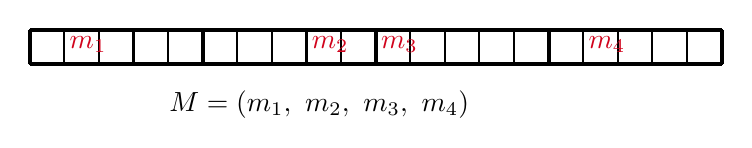
\begin{tikzpicture}[x=0.5pt,y=0.5pt,yscale=-1,xscale=1]
%uncomment if require: \path (0,88); %set diagram left start at 0, and has height of 88

%Shape: Grid [id:dp7159974501706334] 
\draw  [draw opacity=0][line width=0.75]  (15,13) -- (515,13) -- (515,38) -- (15,38) -- cycle ; \draw  [line width=0.75]  (40,13) -- (40,38)(65,13) -- (65,38)(90,13) -- (90,38)(115,13) -- (115,38)(140,13) -- (140,38)(165,13) -- (165,38)(190,13) -- (190,38)(215,13) -- (215,38)(240,13) -- (240,38)(265,13) -- (265,38)(290,13) -- (290,38)(315,13) -- (315,38)(340,13) -- (340,38)(365,13) -- (365,38)(390,13) -- (390,38)(415,13) -- (415,38)(440,13) -- (440,38)(465,13) -- (465,38)(490,13) -- (490,38) ; \draw  [line width=0.75]   ; \draw  [line width=0.75]  (15,13) -- (515,13) -- (515,38) -- (15,38) -- cycle ;
%Straight Lines [id:da4276676225384277] 
\draw [line width=1.5]    (15,38) -- (515,38) ;
%Straight Lines [id:da38414129135222486] 
\draw [line width=1.5]    (15,13) -- (515,13) ;
%Straight Lines [id:da8193193450080452] 
\draw [line width=1.5]    (15,38) -- (15,13) ;
%Straight Lines [id:da4559031610077283] 
\draw [line width=1.5]    (140,38) -- (140,13) ;
%Straight Lines [id:da7340056619830325] 
\draw [line width=1.5]    (515,38) -- (515,13) ;
%Straight Lines [id:da6116177459817139] 
\draw [line width=1.5]    (265,38) -- (265,13) ;
%Straight Lines [id:da4924257748666654] 
\draw [line width=1.5]    (390,38) -- (390,13) ;

% Text Node
\draw (42,16) node [anchor=north west][inner sep=0.75pt]   [align=left] {$\displaystyle \textcolor[rgb]{0.82,0.01,0.11}{m_{1}}$};
% Text Node
\draw (217,16) node [anchor=north west][inner sep=0.75pt]   [align=left] {$\displaystyle \textcolor[rgb]{0.82,0.01,0.11}{m}\textcolor[rgb]{0.82,0.01,0.11}{_{2}}$};
% Text Node
\draw (267,16) node [anchor=north west][inner sep=0.75pt]   [align=left] {$\displaystyle \textcolor[rgb]{0.82,0.01,0.11}{m}\textcolor[rgb]{0.82,0.01,0.11}{_{3}}$};
% Text Node
\draw (417,16) node [anchor=north west][inner sep=0.75pt]   [align=left] {$\displaystyle \textcolor[rgb]{0.82,0.01,0.11}{m}\textcolor[rgb]{0.82,0.01,0.11}{_{4}}$};
% Text Node
\draw (114,55) node [anchor=north west][inner sep=0.75pt]   [align=left] {$\displaystyle M=( m_{1} ,\ m_{2} ,\ m_{3} ,\ m_{4})$};


\end{tikzpicture}
}
\caption{Finding pivot $x$ using median of medians. The median of each subarray~(of size 5) is marked with $m_i$.
We then collect these medians and denote it as $M$. The median of $M$ will be the pivot $x$.}
\label{fig:median}
\end{figure}

There are two questions here. First, how to calculate the median of each subarray?
As each subarray is of size 5, we can use any algorithm. For example, we can sort it, using time of $5 \cdot \log 5$, to get its median.
Note, as there are $n/5$ subarrays, the total running time will be $n/5\cdot 5\cdot \log 5 = \log 5\cdot n = \Theta(n)$.
Second, how to calcuate the median of $M$? The answer is a recursive call: selection~($M$, $|M|/2$).
We will see later on that, the resulting algorithm still runs in linear time.

The pseudo-code for find-pivot function is given below.

\begin{minipage}{0.8\textwidth}
	\aaA {6}{function find-pivot~($A$)}\xxx
	\aab {\textcolor{blue}{if $|A| < 5$: find~(e.g., by sorting $A$) and return the median of $A$;}}\xxx
	\aab {partition $A$ into $n/5$ subarrays of size 5;}\xxx
	\aab {calculate the median of each subarray;}\xxx
	\aab {let $M$ be the array that includes all medians;}\xxx
	\aab {return selection~($M$, $|M|/2$);}\xxx
	\aaa {end algorithm;}\xxx
\end{minipage}

\subsection*{Running Time of the Selection Algorithm}

By definition, the find-pivot functions takes time $\Theta(n) + T(|M|)$.
Therefore, the total running time of the selection problem, in the form of a recurrence,
is $T(n) = \Theta(n) + T(|M|) + \max\{T(|A_1|), T(|A_2|)\}$.

We now bound the size of $|M|$ and $\max\{|A_1|, |A_2|\}$.
Clearly, $|M| = n/5$, as the number of subarrays is $n/5$.
Think: how many numbers in $A$ are \emph{guaranteed} smaller than $x$~(this number then gives a lower bound of $|A_1|$)?
First, in these $n/5$ medians, half of them, i.e., $n/10$ numbers, are smaller than $x$, as $x$ is the median of these medians.
Second, consider these $n/10$ subarrays whose median is smaller than $x$: clearly in each of these subarrays, at least
two numbers are smaller than $x$. This is because the median of this subarray is smaller than $x$ and there are two numbers
in this subarray that are smaller than its median. Combined, we have a lower bound of $|A_1|$: $|A_1| \ge n/10 + 2 \cdot n/10 = 3n/10$.
This gives an upper bound of $|A_2|$: $|A_2| = n - |A_1| \le 7n/10$.

Symmetrically, we have that $|A_2| \ge 3n/10$ and hence $|A_1| = n - |A_2| \le 7n/10$.
This is because, in these $n/5$ medians, $n/10$ of them are larger than $x$,
and in these corresponding $n/10$ subarrays whose median is larger than $x$, there are in total $2\cdot n/10$ numbers larger than $x$.

Combined, we have $\max\{|A_1|, |A_2|\} \le 7n/10$.  The above recurrence becomes $T(n) \le \Theta(n) + T(n/5) + T(7n/10)$.
How to solve this recurrence? Here is the conclusion~(you will see its prove via assignment).
For a more generalized version is this recurrence: $T(n) = \Theta(n) + T(c_1n) + T(c_2n)$, where $0 < c_1, c_2 < 1$, 
we have $T(n) = \Theta(n)$ if $c_1 + c_2 < 1$;
$T(n) = \Theta(n\log n)$ if $c_1 + c_2 = 1$.
For the selection problem we have $c_1 + c_2 = 1/5 + 7/10 < 1$. Hence
its running time $T(n) = \Theta(n)$.

%Therefore, $T(n) = \Theta(n)$ as $1/5 + 7/10 = 9/10 < 1$.

%%\subsection*{Insights about Running Time}
%%
%%Recall that we want to design a linear time algorithm. Let's first have a look at the running time
%%of above algorithm to find a clue what pivot we need to target.
%%Let $T(n)$ be the running time of selection~($A$, $k$) when $|A| = n$. We note that this definition is independent of $k$;
%%in other words, it is the running time for the \emph{worst} choice of $k$.
%%%We \emph{assume} that finding pivot $x$ takes $\Theta(n)$ time.
%%We use $P(n)$ to denote the running time of find-pivot~($A,k$) with $|A| = n$.
%%Partitioning $A$ into $A_1,x,A_2$ clearly takes $\Theta(n)$ time.
%%For the remaining if-else-if-else part, again we assume the \emph{worst-case} scenario, i.e.,
%%the larger array among $A_1$ and $A_2$ will always be chosen.
%%Combined, we have this recurrence: $T(n) = P(n) + \Theta(n) + \max\{T(|A_1|), T(|A_2|)\}$.
%%
%%A good pivot should result in $A_1$ and $A_2$ as balanced as possible. Let's consider two extreme cases.
%%The best case is that $|A_1| = |A_2|$, i.e., $x$ is the median of $A$. In this case, we have $T(n) = \Theta(n) + T(n/2)$.
%%Using master's theorem we have $T(n) = \Theta(n)$.
%%The worst case is that $|A_1| = 0$~(and hence $|A_2| = n - 1$). In this case, we have $T(n) = \Theta(n) + T(n - 1)$.
%%This leads to $T(n) = \Theta(n^2)$.
%%
%%In fact, as long as $\max\{|A_1|, |A_2|\} \le cn$, where $c < 1$, we will have a linear time algorithm.
%%Formally, consider recurrence $T(n) = \Theta(n) + T(cn)$, where $c < 1$. By master's theorem, we know that
%%$T(n) = \Theta(n)$. 


\subsection*{Choices of the Size of Subarrays}

How about we partition $A$ into subarrays of size 3?
Note, in this case the algorithm is still correct.
But will the algorithm still run in linear time?
Let's analyze it.
Now we have $|M| = n/3$, as the number of subarrays is $n/3$.
In these $n/3$ medians, half of them, i.e., $n/6$ numbers, are smaller than $x$,
and in these corresponding $n/6$ subarrays whose median is smaller than $x$, there are in total $1\cdot n/6$ numbers smaller than $x$.
This gives that $|A_1| \ge n/6 + n/6 = n/3$, which gives $|A_2| \le 2n/3$. Symmetrically we can prove $|A_1| \le 2n/3$ and combined we have 
$\max\{|A_1|, |A_2|\} \le 2n/3$.
The recursion in this case, will be $T(n) = \Theta(n) + T(n/3) + T(2n/3)$.
In fact, now $T(n) = \Theta(n\log n)$ as $1/3 + 2/3 = 1$. 
In sum, choosing subarrays of size 3 won't give a linear time algorithm.
(Note: by using the idea of ``median-of-median-of-medians'', a linear-time
algorithm can still be obtained in this case; see assignment.)


How about we partition $A$ into subarrays of size 7?
Now we have $|M| = n/7$, as the number of subarrays is $n/7$.
In these $n/7$ medians, half of them, i.e., $n/14$ numbers, are smaller than $x$,
and in these corresponding $n/7$ subarrays whose median is smaller than $x$, there are in total $3\cdot n/14$ numbers smaller than $x$.
This gives that $|A_1| \ge n/14 + 3n/14 = 2n/7$, which gives $|A_2| \le 5n/7$. Symmetrically we can prove $|A_1| \le 5n/7$ and combined we have 
$\max\{|A_1|, |A_2|\} \le 5n/7$.
The recursion in this case, will be $T(n) = \Theta(n) + T(n/7) + T(5n/7)$.
So $T(n) = \Theta(n)$ as $1/7 + 5/7 < 1$. 
In fact, any odd size that is larger than 5 will lead to a linear-time algorithm.
But bigger size will result in bigger factor in sorting these subarrays. 
For example, compare size of 7 and size of 5: it takes $n/7 \cdot 7 \cdot \log 7 = \log 7 \cdot n$ time to sort in the case of size 7,
which is larger than $\log 5 \cdot n$ in the case of size 5.

\subsection*{Randomized Algorithm for Selection Problem}

We now design a \emph{randomized algorithm} for selection problem.
The idea is simply pick the pivot uniformly at random from $A$.
The pseudo-code is given below.

\begin{minipage}{0.8\textwidth}
	\aaA {2}{function find-pivot-random~($A$)}\xxx
	\aab {pick pivot $x$ uniformly at random from $A$;}\xxx
	\aaa {end function ;}\xxx
\end{minipage}

First, note that the selection algorithm combined with above random function to pick pivot is correct, i.e., it will still find the
$k$-th smallest number of $A$.
We now analyze its running time. 
Again, let $T(n)$ be the running time of selection~($A$, $k$), with above random function to select pivot, when $|A| = n$. 
%Note that $T(n)$ is a random variable, as its running time varies as the choice of the pivot varies.
Define random variable $Z := \max\{|A_1|, |A_2|\}$.
Hence we can write $T(n) = \Theta(n) + T(Z)$.
Again, here $Z$ is a random variable, $T(Z)$ is a random variable, and therefore $T(n)$ is also a random variable.

We aim to calculate the expected running time, a common practice in analyzing randomized algorithms.
We first estimate the distribution of $Z$.
Think: what's the probability for event $Z \le 3n/4$?
Answer: at least $1/2$. Why? This is because we pick $x$ uniformly at random from $x$.
Therefore, the probability of event of $\{x$ is between 25-percentile and 75-percentile of $A\}$ is $1/2$.
And this event is equivalent to the event that $Z \le 3n/4$, according to the definition of $Z$.
Hence, $\Pr(Z \le 3n/4) = 1/2$.

We now calculate its expected running time.
We start with recursion $T(n) = \Theta(n) + T(Z)$.
We first take expectation over $Z$ on both sides: 
$\mathcal{E}_Z [T(n)] = \Theta(n) + \mathcal{E}_Z [T(Z)]$.
Note that $T(n)$ does not contain $Z$~(although $T(n)$ is a random variable), we have 
$\mathcal{E}_Z [T(n)] = T(n)$. That is
$T(n) = \Theta(n) + \mathcal{E}_Z [T(Z)]$.

We now estimate $\mathcal{E}_Z [T(Z)]$.
\begin{eqnarray*}
\mathcal{E}_Z [T(Z)] & = & \sum_{k = n/2}^n \Pr(Z = k) \cdot T(k) \\
 & = & \sum_{k = n/2}^{3n/4} \Pr(Z = k) \cdot T(k)  + \sum_{k = 3n/4}^{n} \Pr(Z = k) \cdot T(k)  \\
 & \le  & T(3n/4) \cdot \sum_{k = n/2}^{3n/4} \Pr(Z = k)  + T(n) \cdot \sum_{k = 3n/4}^{n} \Pr(Z = k)\\
 & =  & T(3n/4) \cdot \Pr(Z \le 3n/4)  + T(n) \cdot \Pr(Z \ge 3n/4)\\
 & \le  & T(3n/4) \cdot 1/2  + T(n) \cdot 1/2.
\end{eqnarray*}

Hence, now we have $T(n) \le \Theta(n) + T(3n/4)/2 + T(n)/2$, which gives $T(n) \le \Theta(n) + T(3n/4)$.
We now take expectation, over $T(n)$, on both sides:
$\mathcal{E}_T [T(n)] = \Theta(n) + \mathcal{E}_T [T(3n/4)]$.
By using master's theorem, we have that $\mathcal{E}_T [T(n)] = \Theta(n)$.
